\documentclass[conference,a4paper]{IEEEtran}
\usepackage{amsmath,amssymb,mathtools}
\usepackage{booktabs}
\usepackage{siunitx}
\sisetup{detect-all, per-mode=symbol}
\DeclareSIUnit{\plato}{\textdegree P}
\DeclareSIUnit{\barg}{bar}
\usepackage{tikz}
\usetikzlibrary{arrows.meta,positioning}
\usepackage{cite}

\newcommand{\degP}{^{\circ}\mathrm{P}}

\title{Research for Improving the Flow-Gain Accuracy of High-Gravity Beer Blending Valves by Using Pressure-Manifold Decoupled Linear Active Disturbance Rejection Control}

\author{%
\IEEEauthorblockN{Thesis draft}%
\IEEEauthorblockA{Automatic control, 2026}%
}

\begin{document}
\maketitle

\begin{abstract}
High-gravity beer is diluted in line by two linear valves whose flows meet in a header, with a third valve setting the header pressure. The flow gain of a linear valve is the installed total derivative along that header, not the partial derivative at frozen pressure, and it moves with the square root of the supply drop. This paper puts the installed gain, computed from measured speeds, stems and pressures, into a first-order linear active disturbance rejection controller as the known coefficient $b_0(t)$. The off-diagonal coupling is left in the total disturbance: the relative-gain array element is only $1.106$, so an inverse decoupler would cancel a ten-percent interaction and replace it with gain noise. A one-line correction of the extended state keeps the stem command continuous when $b_0$ changes. On the design point the installed beer gain is $7.67\,\mathrm{m}^3\mathrm{h}^{-1}$ per unit stem against a partial gain of $12.9$, and using the partial gain would make the command about forty percent too small.
\end{abstract}

\begin{IEEEkeywords}
active disturbance rejection control, control valve, high-gravity blending, relative-gain array, installed gain
\end{IEEEkeywords}

\section{Introduction}
High-gravity brewing ferments a concentrated beer and dilutes it, after fermentation, to the original extract the brand requires \cite{kunze2014brewing,stewart2010highgravity}. On the skid considered here the actuators are three linear control valves: high-gravity beer, deaerated dilution water, and the outlet of the blend header. The fast measurements are the liquid speeds and the supply and header pressures. The extract analyser sits a pipe length downstream and is not used by the flow loops.

Commercial blenders close a flow-ratio loop on the two inlet valves and hold a fixed header pressure \cite{shinskey1996process,seborg2016process}. That structure is correct while the pressure drops stay at the values used to tune it. A linear valve obeys the IEC relation
\begin{equation}
\label{eq:kv}
Q = K_v\, x \sqrt{\frac{\Delta p}{\rho/1000}},
\end{equation}
with $Q$ in cubic metres per hour and $\Delta p$ in bar \cite{iec60534,fisher2005valve}. The gain $\partial Q/\partial x$ therefore falls when a tank head or a pump lowers the supply. At the design point of this skid the beer drop is \SI{1.60}{\barg}. After the beer supply falls from \SI{4.00}{\barg} to \SI{3.05}{\barg} and the header is held, the drop is \SI{0.65}{\barg} and the gain falls by $\sqrt{0.65/1.60}=0.64$. A controller that still divides by the design gain recovers flow too slowly, and the stem runs toward the open stop.

Active disturbance rejection control can absorb an unknown gain error inside an extended state \cite{han2009pid,gao2006paradigm,gao2014centrality}. It does so after the flow has already moved. The pressures that cause the gain change are measured on this skid, so the gain need not be unknown. The contribution of this paper is to put the \emph{installed} gain, the total derivative of flow with respect to stem along the algebraic header balance, into the observer coefficient $b_0$, and to leave the small off-diagonal coupling in the total disturbance rather than invert it.

\section{Installed gain on the pressure manifold}
The header is algebraic on the time scale of the positioners: beer flow plus water flow equals outlet flow,
\begin{equation}
\label{eq:node}
Q_h(x_h,p_h-p_m)+Q_w(x_w,p_w-p_m)-Q_b(x_b,p_m-p_d)=0.
\end{equation}
Differentiating \eqref{eq:kv} at frozen header pressure gives the partial stem gain $Q/x$ for a linear valve. That partial derivative is not the gain the loop sees. Opening the beer valve raises $Q_h$, which raises $p_m$, which reduces the beer drop and also moves the other two flows. The total derivatives along \eqref{eq:node} are fixed by the three pressure sensitivities $S_h=Q_h/(2\Delta p_h)$ and its water and outlet analogues. With $D=S_h+S_w+S_b$,
\begin{align}
G_{hh} &= \frac{Q_h}{x_h}\frac{S_w+S_b}{D}, \label{eq:Ghh}\\
G_{hw} &= -\frac{S_h}{D}\frac{Q_w}{x_w}, \label{eq:Ghw}\\
G_{ww} &= \frac{Q_w}{x_w}\frac{S_h+S_b}{D}. \label{eq:Gww}
\end{align}
Every term on the right is measured: flows from speeds and pipe areas, stems from the positioners, drops from the pressure transmitters. The nominal $K_v$ does not appear. A valve that has lost capacity passes less flow at the same stem, and \eqref{eq:Ghh} reports the gain that the reduced flow implies.

At the design point, $Q_h=\SI{7.50}{\cubic\metre\per\hour}$, $x_h=0.58$, $p_h=\SI{4.00}{\barg}$, $p_m=\SI{2.40}{\barg}$, the partial gain is $Q_h/x_h=12.9$ and the installed gain is $G_{hh}=7.668$. The factor $(S_w+S_b)/D$ equals $0.593$. Using $12.9$ as the controller gain makes every beer command about forty percent too small. The same evaluation gives $G_{hw}=-1.874$, $G_{wh}=-1.580$ and $G_{ww}=4.042$, in cubic metres per hour per unit stem.

The positioner is a first-order lag of time constant $\tau_v=\SI{2.4}{s}$, except inside a stick band of $0.014$ of stem \cite{choudhury2005modelling}. The observer coefficient of the beer loop is therefore the installed gain divided by that time constant,
\begin{equation}
\label{eq:b0}
b_{0,h}(t)=\frac{G_{hh}(t)}{\tau_v}.
\end{equation}
At the design point $b_{0,h}(0)=7.668/2.4=3.195$. The water coefficient is $4.042/2.4=1.684$. A command step of $0.1$ must produce an initial beer-flow derivative of $0.320\,\mathrm{m}^3\mathrm{h}^{-1}\mathrm{s}^{-1}$. That derivative is the acceptance test of \eqref{eq:Ghh}.

Three protections keep the division honest. Stems below $0.05$ and pressure drops below \SI{0.12}{\barg} are replaced by those floors, because a shut valve has no meaningful $Q/x$ and a vanishing drop sends $S$ to infinity. The resulting $b_0$ is filtered with a time constant of \SI{2.5}{s}, slower than the flow loop and faster than a tank-head change.

\section{Why the interaction is not inverted}
The relative gain of the beer--water pair is
\begin{equation}
\lambda_{11}=\left(1-\frac{G_{hw}G_{wh}}{G_{hh}G_{ww}}\right)^{-1}=1.106.
\end{equation}
Bristol's measure says that a diagonal controller already sees within about ten percent of the fully decoupled gain \cite{bristol1966rga,skogestad2005multivariable}. An inverse decoupler would cancel the fraction $G_{hw}G_{wh}/(G_{hh}G_{ww})=0.0955$ and would replace it with the error of the gain estimates. Those estimates are noisy at the level of the flow transmitters, and they are wrong while a valve is stuck, because $Q/x$ during a stick interval does not describe the impending slip. The off-diagonal terms therefore stay inside the total disturbance. A water-command move changes beer flow within one positioner time constant, the beer observer sees the flow error, and the extended state cancels it. The cost is a transient of a fraction of a second. The benefit is that a wrong $G_{hw}$ cannot push the beer valve.

\section{Observer, control law, and a continuous command}
For the beer loop the linear extended-state observer and the control law are the bandwidth form of Gao \cite{gao2003scaling,fu2016tuning},
\begin{align}
\dot{z}_1 &= z_2 + b_{0,h} u_h + 2\omega_o(Q_h-z_1), \label{eq:z1}\\
\dot{z}_2 &= \omega_o^2(Q_h-z_1), \label{eq:z2}\\
u_h &= \mathrm{sat}_{[0.02,0.98]}\!\left(\frac{\omega_c(Q_h^\star-z_1)-z_2}{b_{0,h}}\right). \label{eq:u}
\end{align}
The water loop is the same observer with its own states. The command that re-enters \eqref{eq:z1} is the command after a \SI{0.40}{s} filter, which is the command the positioner actually received. If the valve is on the limit, $z_2$ explains the flow that the limited command produces and does not wind \cite{han2009pid,astrom2006advanced}.

The bandwidths are $\omega_c=0.85$ and $\omega_o=2.5$ radians per second. The ratio $\omega_o/\omega_c\approx 3$ is at the low end of the usual range \cite{gao2003scaling,herbst2013simulative}. It is acceptable because $f$, the total disturbance, no longer contains the square-root pressure term, so its derivative is smaller and a modest $\omega_o$ still keeps the observation error small \cite{guo2011convergence,huang2014methodology}. The transfer function from flow noise to $z_2$ is $\omega_o^2 s/(s+\omega_o)^2$. With a flow-meter standard deviation of \SI{0.012}{\cubic\metre\per\hour}, raising $\omega_o$ from $2.5$ to $8$ produces command noise that the stick band does not hide.

While $z_2$ tracks $f$ and the command is not saturated, the closed loop collapses to $\dot{Q}_h=\omega_c(Q_h^\star-Q_h)$. A throughput ramp of \SI{1.5}{\cubic\metre\per\hour} in \SI{20}{s} then lags by $0.075/0.85=\SI{0.088}{\cubic\metre\per\hour}$, about one percent of the design flow, independent of the supply pressure. That separation is the point of putting the pressure into $b_0$.

The same controller is an integral controller in internal-model form when $b_0$ is constant \cite{tan2016imc}. Scheduling $b_0$ must not break the integral state. Let $S=z_2+b_0 u$. Replacing $b_0$ at fixed $z_2$ changes $S$ by $\Delta b\cdot u$ and the command jumps. The correction, applied before the observer step,
\begin{equation}
\label{eq:inv}
z_2^+ = z_2 + (b_0-b_0^+)\,u,
\end{equation}
holds $S$ constant. Its size is concrete. At $u_h=0.70$ with $b_0=3.20$, equilibrium gives $z_2=-2.24$. Replacing $b_0$ by the high-rate installed value $3.97$ without \eqref{eq:inv} returns $u_h^+=2.24/3.97=0.56$, a fall of $0.14$ of stem in one sample, far outside the stick band of $0.014$. With \eqref{eq:inv}, $z_2^+=-2.78$ and $u_h^+=0.70$. The stem does not move.

Initial conditions use the same identity. At the design stem, $z_2(0)=-3.195\times 0.58=-1.853$, so \eqref{eq:u} reproduces $u_h(0)=0.58$. Starting from $z_2=0$ invents a disturbance and walks the valve off the design point.

\begin{figure}[!t]
\centering
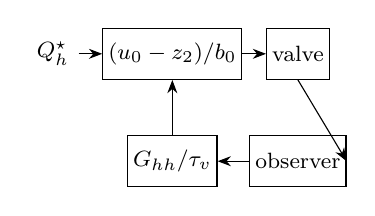
\begin{tikzpicture}[>=Stealth, node distance=4mm, font=\footnotesize,
  blk/.style={draw, minimum height=6.5mm, inner sep=2pt, align=center}]
  \node (r) {$Q_h^\star$};
  \node[blk, right=3mm of r] (law) {$(u_0-z_2)/b_0$};
  \node[blk, right=3mm of law] (v) {valve};
  \node[blk, below=7mm of law] (g) {$G_{hh}/\tau_v$};
  \node[blk, below=7mm of v] (eso) {observer};
  \draw[->] (r) -- (law);
  \draw[->] (law) -- (v);
  \draw[->] (v.south) -- (eso.east);
  \draw[->] (eso.west) -- (g.east);
  \draw[->] (g.north) -- (law.south);
\end{tikzpicture}
\caption{One inlet loop. The installed gain is measured. The other inlet valve enters only through the plant.}
\label{fig:loop}
\end{figure}

Figure~\ref{fig:loop} is one inlet loop. Nothing in the figure crosses to the other loop except through the plant. The structure is two function blocks \cite{madonski2019error,wu2021transition}.

\section{What the campaign shows about the gain}
The flow loops of this paper are estimated together with a header coordinator and an extract soft sensor, reported in the companion paper, against ratio proportional--integral control and against linear active disturbance rejection control that freezes $b_0$ at the design value. The campaign lasts \SI{560}{s} and includes a beer-supply step from \SI{4.00}{\barg} to \SI{3.05}{\barg}, a water-supply oscillation, a brand change, a throughput rise to \SI{9}{\cubic\metre\per\hour}, a hidden mother-beer drift and a ten-percent loss of beer-valve $K_v$. The three controllers share one noise draw.

The full-run beer-flow integrals are $286$, $316$ and $37.5\,\mathrm{m}^3\mathrm{h}^{-1}\mathrm{s}$ for proportional--integral control, frozen-gain active disturbance rejection and the proposed pair. The two baselines finish with the beer stem near the stop at $0.98$ and a beer flow near \SI{7.4}{\cubic\metre\per\hour}. The proposed beer flow at the same instant is \SI{9.06}{\cubic\metre\per\hour}, with the stem at $0.77$. That gap is joint: the coordinator of the companion paper restores the pressure drop, and the gain of this paper keeps the command matched to the drop that remains.

The part that belongs to $b_0(t)$ can be seen before the stem reaches the stop. On the supply step, with the header still near its old value, a frozen $b_0$ overstates the gain, the cancellation in \eqref{eq:u} is too large, and the effective bandwidth falls. The beer-flow integral on that \SI{80}{s} window is $14.0$ for the frozen observer and $12.8$ for the scheduled gain. The proportional--integral loop, stiff at the old gain, integrates only $7.7$, at the price of driving the beer stem to $0.91$. Later, at \SI{9}{\cubic\metre\per\hour} and a header of \SI{1.45}{\barg}, the installed beer gain has risen from $7.67$ to $9.53$, so $b_{0,h}=3.97$ against the frozen $3.20$. The frozen coefficient then understates the gain and the command is about a quarter too large. Table~\ref{tab:pts} collects the two operating points. The partial gain happens to be $12.9$ at both, which is why a partial-gain design cannot see that the plant has changed.

\begin{table}[!t]
\caption{Beer-loop coefficients at the two operating points.}
\label{tab:pts}
\centering
\begin{tabular}{@{}lcc@{}}
\toprule
Quantity & Design & High rate \\
\midrule
Header (\si{\barg}) & 2.40 & 1.45 \\
Partial gain $Q_h/x_h$ & 12.9 & 12.9 \\
Installed gain $G_{hh}$ & 7.67 & 9.53 \\
$b_{0,h}$ & 3.20 & 3.97 \\
$\lambda_{11}$ & 1.106 & 1.026 \\
\bottomrule
\end{tabular}
\end{table}

\section{One sample, and the gain the header decides}

The same identities can be checked on a single sample of \SI{10}{ms}. Start at the design point, $b_{0,h}=3.195$, $z_1=7.50$, $z_2=-1.853$, $u_h=0.58$. The measured flow then steps to \SI{7.40}{\cubic\metre\per\hour} because the supply has fallen, and the gain update has already moved $b_{0,h}$ to $2.70$. Equation~\eqref{eq:inv} first replaces the disturbance estimate by
\begin{equation}
z_2 = -1.853+(3.195-2.70)\times 0.58 = -1.566,
\end{equation}
and $z_2+2.70\times 0.58$ remains zero, so the command does not jump because the gain changed. The observer error is $7.40-7.50=-0.10$. One Euler step moves $z_1$ by $-0.005$ and $z_2$ by $-0.00625$. The new command is
\begin{equation}
u_h=\frac{0.85(7.50-7.495)-(-1.572)}{2.70}=0.584.
\end{equation}
The stem opens by a few thousandths in that sample. While the flow error persists, $z_2$ accumulates at $\omega_o^2 e$, and the denominator is already the new gain. The frozen-gain controller divides the same $z_2$ by $3.195$ and therefore produces a smaller command. That one-sample difference is the fixed-gain baseline of the comparison.

Table~\ref{tab:path} evaluates \eqref{eq:Ghh} after the beer supply has fallen to \SI{3.05}{\barg}, with the design flows restored by whatever stem \eqref{eq:kv} then requires. The partial gain ignores the header. The installed gain is the one \eqref{eq:b0} must use.

\begin{table}[!t]
\caption{Beer-valve gain after the supply falls to \SI{3.05}{\barg}, design flows restored.}
\label{tab:path}
\centering
\begin{tabular}{@{}lccc@{}}
\toprule
Header (\si{\barg}) & Stem & Partial $Q_h/x_h$ & $G_{hh}$ \\
\midrule
2.40 & 0.91 & 8.24 & 3.06 \\
1.80 & 0.66 & 11.4 & 6.88 \\
1.71 & 0.63 & 11.8 & 7.49 \\
\bottomrule
\end{tabular}
\end{table}

The first row is a fixed header. The stem is already at the edge of the linear window and $G_{hh}$ has fallen from $7.67$ to $3.06$. A controller that keeps the design $b_0$ divides by more than twice the true gain, so the same observer state produces less than half the stem movement the flow error calls for. The third row is the header the companion coordinator selects at this supply. The stem is back near $0.63$ and $G_{hh}=7.49$ is close to the design value. The difference between those rows is why an outlet valve belongs in the flow problem. It is not solved by a better $b_0$ alone.

The static inverse can be written down and then set aside. With the design gains, $\det G=7.668\times 4.042-(-1.874)(-1.580)=28.04$. The diagonal elements of $G^{-1}$ are $0.144$ and $0.274$, against $1/G_{hh}=0.130$ and $1/G_{ww}=0.247$. The relative correction is about ten percent, which is $\lambda_{11}-1$. An inverse whose gains are wrong by a stick band of $0.014$, about $2.4$ percent of the design beer stem and rather more of the flow while the valve is stuck, feeds that error into both loops with the off-diagonal sign. The ten percent is left in the total disturbance, where a wrong sign cannot move the other valve \cite{morari1989robust,chen2016dobc}.

Subtracting the observer from the plant, when $b_{0,h}$ equals the true coefficient and varies slowly, gives an error system whose characteristic polynomial is $(s+\omega_o)^2$. The forced error in $z_2$ is of order $|\dot{f}|/\omega_o$ \cite{guo2011convergence,khalil2002nonlinear}. A Lyapunov function for the unforced error is $V=\omega_o^2\tilde{z}_1^2+\tilde{z}_2^2$, and $\dot{V}=-2\omega_o^3\tilde{z}_1^2$ when $\dot{f}=0$. The known-gain term is what keeps $|\dot{f}|$ small enough for $\omega_o=2.5$. Without it, $\dot{f}$ during the supply step contains the derivative of a square-root gain, and the observer would have to be faster than the noise budget allows.

\section{Ratio setpoints, oscillation, and a loss of capacity}
The beer-flow setpoint is the production rate. The water-flow setpoint is $Q_w^\star=R Q_h^\star$, with $R$ taken from the extract controller of the companion paper, equal to $0.338$ at the design extract of \SI{12}{\plato}. Using the beer setpoint rather than the measured beer flow is the ratio-on-setpoint rule \cite{shinskey1996process}. A noise spike on the beer speed then does not move the water valve. During a throughput ramp both setpoints move in proportion, and both installed-gain observers track them through $\dot{Q}=\omega_c(Q^\star-Q)$.

The water-supply oscillation is the test of a gain that is measured rather than observed. From \SI{130}{s} to \SI{210}{s} the water supply moves with amplitude \SI{0.28}{\barg} and period \SI{26}{s}. It enters $G_{ww}$ through $\Delta p_w$ on the sample it occurs, and $b_{0,w}$ follows through the \SI{2.5}{s} filter. Extract integrals on the window are $3.40$, $3.64$ and $2.02\degP\cdot\mathrm{s}$ for proportional--integral control, the frozen observer and the scheduled gain. Beer-flow integrals are $6.62$, $10.2$ and $4.89$. Peak extract errors are $0.109$, $0.140$ and $0.086\degP$. The frozen observer does reject the oscillation, which is why the extract error stays near a tenth of a degree, but the rejection is late by a fraction of $\omega_o$ and the peak is the largest of the three. The scheduled coefficient has already moved before $z_2$ is asked to.

A ten-percent loss of beer-valve $K_v$ at \SI{480}{s} is not announced. Equation~\eqref{eq:Ghh} does not need the announcement: the valve passes less flow at the same stem, $Q_h/x_h$ falls, and $b_{0,h}$ falls with it. On the last \SI{80}{s} the beer-flow integrals are $121$, $135$ and $4.60\,\mathrm{m}^3\mathrm{h}^{-1}\mathrm{s}$. The two baselines are already on the open stop from the throughput ramp, so a further loss of capacity has nowhere to go. The scheduled loop is at a stem near $0.77$, inside the stroke, and the flow error stays at the level of the earlier windows. The formula's refusal to use the nameplate $K_v$ is what makes that last window a gain test rather than a saturation test.

\section{Design choices that were rejected}
Several neighbouring designs were computed and then not used. They are recorded because each one is the version a first implementation tends to build.

An inverse decoupler was the first. Section above gives its diagonal. Feeding the off-diagonal of $G^{-1}$ forward, even at a fraction of its value, produced a limit cycle from the first second: each valve's command moved the other's flow, the observers corrected, and the stick bands turned the correction into a slip. Travel of several tens of stem-units over the run followed, against a travel near zero in the undisturbed first minute of the retained design. The relative gain $1.106$ is the reason the cycle is not worth the ten percent it would cancel in the steady state.

A fast gain filter was the second. Passing $b_0$ through a \SI{0.45}{s} filter, and writing the new gain into the observer without \eqref{eq:inv}, made the command jump on every noisy update of $Q/x$. The stick band then released and recaptured continuously. The retained filter is \SI{2.5}{s}, and \eqref{eq:inv} is applied before the observer step, using the command the positioner actually received. The command filter of \SI{0.40}{s} is that received command. Using the unlimited command instead lets $z_2$ integrate a move the valve did not make.

A partial-gain $b_0$ was the third. At the design point $Q_h/x_h=12.9$ and $G_{hh}=7.67$. The controller that divides by $12.9/\tau_v$ issues commands about forty percent too small at the one point where the plant was identified, and it has no signal that tells it so, because the partial derivative never sees $p_m$ move. Table~\ref{tab:path} is the same mistake at the reduced supply: the partial column and the installed column are not interchangeable at any row.

The bandwidths themselves have a sequence that does not search the scenario. Identify $\tau_v$ from a stem step in manual, and confirm $G_{hh}$ from the initial flow derivative after a small step. Set $\omega_c$ near $2/\tau_v$ only after that derivative matches \eqref{eq:b0}; otherwise lower it. Set $\omega_o\approx 3\omega_c$ and read the stem travel over a quiet minute. Travel that is not zero means the command is crossing the stick band, and the remedy is a lower $\omega_o$ or a corrected $b_0$, not a faster observer. The flow loops of this paper stop at that test. The header bandwidth, the dead zone and the extract bandwidth belong to the companion paper, and they are required to stay slower than $\omega_c=0.85$. A header loop placed in the same band as these flow loops oscillates against them. The oscillation is not a defect of \eqref{eq:Ghh}.

\section{Conclusion}
The inlet valves of a high-gravity blender are linear, but their loop gain is the installed gain along the header balance, and that gain is a function of measured pressures and measured flows. Writing it into $b_0$, filtering it, and correcting $z_2$ when it changes removes the supply pressure from the total disturbance without inverting a relative gain of $1.11$. The extended state is left with stiction, the small off-diagonal coupling, and whatever the gain formula has not yet followed. The header setpoint that keeps those valves off the stop, and the delayed soft sensor that trims the extract, are the subject of the companion paper. Neither paper replaces the other: a correct $b_0$ does not create drop that a nearly open valve no longer has.

\bibliographystyle{IEEEtran}
\bibliography{refs}

\end{document}
